
\section{Introdução}\label{sec-introdução}
Iniciamos este artigo explicitando uma antiga percepção compartilhada e,
frequentemente, provocada ao dialogarmos com comunidades escolares e ao
transitarmos por tais instituições. Referimo-nos às morosas mudanças em
aulas ministradas em escolas de ensino básico, que se encontram na
contramão de transformações constantemente demandadas na sociedade. A
inovação do ensino ocorre lentamente e, talvez, torne-se mais
perceptível, ainda que compreendida de forma restrita, quando se
visualiza o trabalho realizado por educadores de diferentes gerações.

Neste artigo, contrapomo-nos à concepção restrita de inovação sinalizada
na fronteira mencionada entre gerações. Tal concepção se caracteriza
pela instauração de ``fronteiras nítidas e firmes entre a inovação e o
conservadorismo, ou entre o inovador e o tradicional'' \cite[p. 8]{signorini_apresentacao_2007}. Ainda nos termos de \textcite[p. 8]{signorini_apresentacao_2007}, o que, efetivamente,
compreendemos por inovação se instaura em ``bordas fluidas e dinâmicas,
ou seja, zonas de contínuo embaralhamento do que
\phantomsection\label{anchor-2}{}se apresenta como separado e excludente
nos discursos de autoridade sobre língua(gem) e ensino''\footnote{
	\phantomsection\label{anchor-3}{}Destacamos ainda os seguintes termos
	da autora: ``essas zonas de embaralhamento entre princípios
	teórico-metodológicos diversos e práticas de ensino também diversas
	são espaços dinâmicos, sempre em processo de mudança, mais ou menos
	acelerada, mais ou menos disruptiva, em relação ao centro, e mais ou
	menos produtiva do ponto de vista da inovação. Isso porque as
	transformações são sempre moleculares e em direções variadas, não
	necessariamente correspondem às da demanda que desencadeou o processo,
	ou às que pretendiam os atores sociais envolvidos'' \cite[p. 8]{signorini_apresentacao_2007}.}.



Subjacente ao ambiente escolar resistente à inovação, encontra-se o
provável desconhecimento de que saberes especializados, passíveis de uso
em aulas de diferentes componentes curriculares, são produzidos
ininterruptamente em distintos campos do conhecimento, a exemplo da
Linguística Aplicada (LA), campo em que esta pesquisa se encontra
situada. Assim, o aprimoramento profissional de professores, como o de
qualquer outra categoria, deve ser constante e a obtenção do primeiro
diploma universitário não pode se configurar como uma credencial única e
definitiva.

Este artigo mostra um recorte de resultados de uma investigação
científica qualitativa, caracterizada por um planejamento colaborativo,
seguido por uma intervenção pedagógica, com propósito principal de
inovar o estudo da gramática, em aulas de Português como língua materna,
em escolas públicas brasileiras de Ensino Fundamental. Está vinculada ao
projeto Conscientização Gramatical pela Educação Científica
(ConGraEduC)\footnote{O projeto foi aprovado pelo Comitê de Ética em
	Pesquisa da UFT, sob o parecer 3.457.383.}, aprovado em uma chamada
pública para pesquisadores, vinculada ao Programa Ciência na Escola
(PCE), financiado pelo governo federal brasileiro, com propósito de
inovar o ensino e de proporcionar uma formação discente crítica a partir
da abordagem por nós denominada de educação científica\footnote{Na
	Chamada Pública MCTIC/CNPq Nº 05/2019 -- Programa Ciência na Escola,
	objetiva-se contribuir com ``ensino de ciências na educação básica, em
	consonância com o Objetivo do Desenvolvimento Sustentável -- ODS 4:
	\emph{Educação de Qualidade}'' \cite[1 - Objetivo]{brasil_chamada_2019}. Também se
	apresenta como objetivo da chamada a promoção de aproximação entre as
	instituições de ensino básico e superior, ``devendo privilegiar o
	letramento científico, o uso de abordagens investigativas e de
    	metodologias ativas de ensino'' \cite[item 1.1.1]{brasil_chamada_2019}.}. O projeto
ainda contribui para as investigações científicas desenvolvidas no grupo
de pesquisa Práticas de Linguagens -- PLES (CNPq/UFT).



Este estudo foi caracterizado como uma pesquisa baseada em
\emph{design}, conforme concepção assumida por \textcite{anderson_design-based_2012}, ao caracterizar o percurso investigativo marcado pelo
planejamento interventivo e colaborativo e informado por pressupostos
teóricos, em função da transformação do ensino e do fortalecimento da
teoria. Sob a influência do próprio programa de fomento à pesquisa e de
formação de pessoal, a principal abordagem teórica utilizada foi a da
educação científica, em desenvolvimento na LA \cite{freitas_educacao_2022,magalhaes_formacao_2023,silva_educacao_2020a,silva_educacao_2023}. Essa abordagem informou o
planejamento interventivo, marcado pela elaboração e testagem de
materiais de ensino, a exemplo de jogos didáticos focalizados mais
diretamente neste artigo. Auxiliou a construção colaborativa de
procedimentos pedagógicos diferenciados.

O ensino improdutivo de gramática ainda se configura como um dos maiores
desafios das aulas de língua materna, pois o trabalho escolar de
reprodução e memorização de metalinguagem e de conceitos gramaticais
continua se retroalimentando, pouco contribuindo para a formação de
leitores e escritores \cite{silva_construcao_2019}. Esse diagnóstico
pode até ser realizado por educadores em seus locais de trabalho, mas as
soluções para minimizar ou resolver o desafio estão por ser elaboradas.
Não nos interessa menosprezar o dinamismo e a relevância da cultura
escolar, até porque, conforme dito, esta pesquisa foi realizada a partir
do trabalho conjunto entre professoras da escola básica e docentes do
ensino superior, parceria marcada pela (re)construção de saberes e,
inclusive, na própria autoria deste artigo\footnote{ Optamos por
	utilizar professoras, no gênero feminino, para fazer referência a
	profissionais da escola básica participantes do projeto, pois, durante
	a primeira etapa focalizada de trabalho, conforme explicitado na seção
	seguinte, os dois professores precisaram se ausentar do grupo.}.

Este artigo está organizado em quatro principais seções, além desta
Introdução, das Considerações finais e das Referências. Em ``Percurso
metodológico construído'', situamos a investigação compartilhada no
campo da Linguística Aplicada e caracterizamo-la como uma pesquisa
baseada em \emph{design}. Em ``Análise linguística na perspectiva da
educação científica'', sintetizamos os principais fundamentos teóricos
utilizados neste recorte investigativo. Em ``Jogo como instrumento lúdico de mediação do aprendizado'', descrevemos o
material didático digital focalizado e exemplificamos como ele pode
contribuir para um estudo produtivo da gramática. Finalmente, em
``Transformação em aula de língua materna'', apresentamos mudanças de
representações discentes sobre aulas de Língua Portuguesa (LP),
gramática, ciência e pesquisa, a partir da análise comparativa de
entrevistas realizadas antes e depois da intervenção pedagógica.

\section{Percusso metodológico construído}\label{sec-Percussometodológicoconstruído}

Uma concepção indisciplinar de LA foi assumida nesta investigação,
caracterizada pelo uso de pressupostos teóricos de diferentes
disciplinas ou campos do conhecimento para subsidiar a elaboração de
resposta ao seguinte objetivo de pesquisa: descrever uma estratégia
inovadora de ensino de língua materna mediada pelo uso do jogo digital
Gramática das Fábulas. O compromisso com contribuições formativas para
os envolvidos na pesquisa e a visibilização de vozes periféricas ou
marginais também caracterizam a concepção mencionada de LA.

O jogo didático auxiliou os estudantes colaboradores a reconhecerem e a
compreenderem o funcionamento de elementos da gramática da oração,
incluindo aí a composição de grupos gramaticais realizados abaixo do
nível oracional. Assim, enfatizamos o sistema de TRANSITIVIDADE da
oração, numa perspectiva sistêmico-funcional da gramática, conforme
detalhado na seção seguinte. A abordagem gramatical da linguística
sistêmico-funcional (LSF) \cite{eggins_introduction_2004,halliday_hallidays_2014} e
a pedagógica da educação científica \cite{silva_letramento_2016,silva_educacao_2020a, silva_educacao_2023} integraram os principais referenciais utilizados na produção e na
implementação do referido material didático, bem como na análise de
dados neste artigo.

A identificação desta investigação como uma \emph{pesquisa baseada em
	design} (PBD) se justifica pela necessidade de produção (a) de
conhecimento pedagógico para o estudo da gramática em aulas de língua
materna; e (b) de conhecimentos teóricos sobre a abordagem da educação
científica no ensino e na formação de professores da referida língua, na
perspectiva assumida da LA. Nesse sentido, interessou-nos uma produção
colaborativa entre professores da escola básica e docentes
universitários, gerando-se resultados mais duradouros ou sustentáveis
diante das demandas mencionadas. Podemos questionar o que justificaria o
alcance de resultados sustentáveis a partir do trabalho colaborativo
entre os referidos educadores. Os seguintes termos de \textcite{anderson_design-based_2012} formulam uma resposta possível para tal questionamento:
\begin{quote}
A parceria em um estudo baseado em \emph{design} reconhece que os
professores geralmente estão muito ocupados e, muitas vezes, mal
treinados para realizar pesquisas rigorosas. Da mesma forma, o
pesquisador, muitas vezes, não conhece as complexidades da cultura,
tecnologia, objetivos e políticas de um sistema educacional para criar e
medir efetivamente o impacto de uma intervenção. Assim, desenvolve-se
uma parceria que negocia o estudo desde a identificação inicial do
problema, passando pela revisão da literatura, até ao design de
intervenção, construção, implementação, avaliação, e até à criação e
publicação de princípios teóricos e de \emph{design} \cite[p. 17]{anderson_design-based_2012}.
\end{quote}


Os autores mencionados elencam o que podemos compreender como oito
princípios caracterizadores da PBD: situa-se em um contexto educacional
real; focaliza o \emph{design} e o teste de uma intervenção
significativa; utiliza metodologias mistas (incluindo aí diferentes
instrumentos e estratégias de geração de dados); envolve múltiplas
interações em função dos diferentes participantes; envolve parcerias
colaborativas entre pesquisador e agente da prática profissional;
realiza-se no dinamismo de princípios do \emph{design} conforme contexto
de implementação; compara-se à pesquisa-ação e dela diferencia-se pelo
enfoque teórico e parceria interinstitucional; impacta de forma prática
o fazer laboral efetivo \cite{anderson_design-based_2012}.



O trabalho compartilhado neste artigo corresponde à primeira etapa do
ConGraEduC, caracterizada por bastante instabilidade no roteiro de
atividades, provocada pelo surgimento intempestivo da pandemia do
coronavírus SARS-CoV-2. Assim, as reuniões de pesquisa entre educadores,
as aulas ministradas e as orientações de estudantes ocorreram
predominantemente na modalidade remota, entre abril de 2020 e julho de
2022. Todas foram gravadas em vídeo com a plataforma virtual
\emph{Zoom}. No segundo semestre de 2019, foram realizadas as primeiras
reuniões presenciais de pesquisa, sem registros em áudio ou vídeo.
Posteriormente, o uso desses recursos foi facilitado com a adesão ao
trabalho remoto. A segunda etapa será planejada após a conclusão das
investigações em andamento sobre os dados gerados. Na ocasião,
pretendemos realizar intervenções em aulas presenciais do ensino básico
regular, com outros professores voluntários e com os interessados em
permanecer no projeto.



Na primeira etapa do projeto, as pessoas envolvidas foram organizadas em
uma equipe pedagógica, vinculada à Universidade Federal do Tocantins
(UFT), instituição sede do projeto, e em uma equipe técnica, vinculada
ao Instituto Federal do Tocantins (IFTO), instituição parceira. A
primeira foi formada por mestrandos, doutorandos e docentes do ensino
superior, responsáveis pela criação de diferentes materiais didáticos e
pelo planejamento de intervenções pedagógicas. A segunda equipe foi
formada por um coordenador com formação em sistemas de informática e
três bolsistas de iniciação científica, sendo um de nível superior e
outros dois de nível médio técnico, responsáveis pela programação de
dois jogos digitais de trilhas (Trilha do Sítio; Trilha do Visconde) e
pelo trabalho de consultoria para a idealização e o desenvolvimento do
Laboratório Virtual de Pesquisa Escolar com Gramática (LabGram),
disponível em:
\url{http://www.wagnerodriguesilva.com.br/labgram}.



A composição dessas equipes passou por mudanças durante o
desenvolvimento do projeto, algumas consideradas bastante
significativas, escapando ao que compreendemos que sejam alterações
naturais em trabalhos desse tipo, conforme tematizado por \textcite{silva_desafios_2023}. Inicialmente, a primeira equipe era composta por
cinco professoras da escola básica com vínculo em curso de doutorado, um
mestrando com vínculo de servidor técnico na instituição sede, além de
dois docentes vinculados à instituição sede, sendo um coordenador do
projeto e uma terceira docente servidora de outra instituição
universitária parceira. As duas docentes precisaram deixar o projeto no
período pandêmico, e dois doutorandos desistiram do curso por questões
de foro íntimo. Já no final dos estágios de elaboração de material
didático e de intervenção propriamente dita, uma doutoranda com vínculo
de professora da escola básica ingressou na equipe, além de três
mestrandas, sendo uma professora da escola básica e duas egressas do
Programa Institucional de Iniciação Científica (PIBIC).\textsuperscript{
}As teses de doutorado e a dissertação de mestrado foram ou estão sendo
desenvolvidas dentro do ConGraEduC \cite{antonella_recontextualizacao_2023,ribeiro_producao_2021}.



O percurso da primeira etapa pode ser descrito em três principais
estágios de configuração do \emph{design} da pesquisa, os quais se
sobrepõem em diferentes momentos: 
\begin{enumerate}
	\item Reuniões de pesquisa para estudo de teorias orientadoras dos trabalhos característicos dos demais estágios, para produção de materiais didáticos e planejamento de situações educativas;
	
	\item Intervenções pedagógicas realizadas com estudantes de escolas públicas;\footnote{Foram iniciadas intervenções pedagógicas em turmas do Ensino Fundamental II no Pará (PA) e no Tocantins (TO), estados da Região Norte do Brasil. Porém, em função de adversidades pessoais no percurso, dois professores interromperam as intervenções nas próprias salas de aula e desistiram do doutorado. Apenas a intervenção realizada no Estado do Pará foi concluída, a qual é focalizada diretamente neste artigo. Os materiais didáticos produzidos são/foram utilizados em formações continuadas na rede pública de ensino do Município de Imperatriz, Estado do Maranhão, conforme mostraram \textcite{silva_educacao_2023}.}.
	\item Trabalho de análise dos dados gerados e de divulgação dos resultados em diferentes gêneros acadêmicos e situações interativas.
\end{enumerate}

Nas reuniões de pesquisa, foram estudadas as abordagens da LSF, das
metodologias ativas e da educação científica, sempre no esforço de
identificar e compreender categorias e conceitos relevantes ao projeto,
os quais auxiliaram o trabalho colaborativo de elaboração de materiais
didáticos integrantes do LabGram, conforme descrito em \textcite{silva_desafios_2023}. Para tanto, foram produzidos 53 textos didáticos, 53
vídeos didáticos, 13 jogos didáticos com suas respectivas versões
analógicas e uma unidade didática para orientar as intervenções
pedagógicas das professoras em suas respectivas salas de aula \cite{ribeiro_professores_2021, silva_construcao_2021}.



Ainda sobre as intervenções pedagógicas, as atividades de ensino com
pesquisa, focalizadas diretamente neste artigo, aconteceram em uma
escola urbana de Conceição do Araguaia, no interior do Pará, na região
amazônica brasileira. Na ocasião, foram realizadas aulas remotas e
presenciais, sendo essas últimas ministradas para grupos com frequência
alternada na escola, em função do rodízio de estudantes no período
pandêmico. Essa foi a alternativa adotada pela instituição para evitar
ambientes fechados com pessoas vulneráveis ao SARS-CoV-2.



Por conta dessas circunstâncias e de outras particularidades típicas das
escolas de ensino básico e das próprias pesquisadoras, o trabalho
interventivo abrangeu, aproximadamente, dois semestres letivos
subsequentes em anos letivos distintos -- 2º semestre de 2021 e 1º
semestre de 2022. As primeiras particularidades corresponderam à
aplicação de simulados e avaliações públicas de larga escala para
averiguar o rendimento dos estudantes, atividades extras e eventos
constitutivos do calendário institucional, além da resistência de
professoras da escola ao trabalho diferenciado proposto. As segundas
corresponderam à sobrecarga de trabalho de uma das participantes, sem
afastamento de qualificação para realização do doutorado, e à
participação remota da segunda professora, que morava em outro estado.

Na intervenção focalizada, uma média de 30 estudantes do 9º ano do
Ensino Fundamental II se envolveram como colaboradores. Em decorrência
das instabilidades na retomada das aulas presenciais, alguns desses não
frequentavam a escola assiduamente\footnote{ Inicialmente, a intervenção
	foi idealizada para ser realizada com os referidos colaboradores no
	então segundo semestre do 7º ano, conforme escolha da professora
	participante servidora da instituição, porém houve um significativo
	atraso no planejamento da pesquisa e, posteriormente, em decorrência
	da pandemia, resultando na intervenção junto aos estudantes já no 9º
	ano. As atividades da intervenção foram realizadas com morosidade,
	havendo necessidade de mais tempo para integralização, o que
	justificou a finalização do trabalho no primeiro semestre letivo do
	ano seguinte, com os estudantes dispersos em diferentes turmas do 1º
	ano do Ensino Médio, funcionando na modalidade de ensino integral, na
	ocasião, implementado na escola.}. Os desafios se intensificaram
quando a instituição passou a ofertar a modalidade integral do Ensino
Médio. Vários remanescentes do referido 9º ano integraram diferentes
turmas de 1ª série da escola, no semestre subsequente, dificultando o
trabalho de intervenção.



Nessa etapa final, a situação demandou a realização de encontros remotos
com pequenos grupos de estudantes para a orientação e o desenvolvimento
de oficinas de produção de textos orais e escritos, e de análise de
registros da pesquisa escolar. Nesse contexto, foram gerados diferentes
dados passíveis de cruzamento numa abordagem analítica qualitativa, em
diferentes recortes investigativos, sob a responsabilidade de
professoras participantes e do docente coordenador. Os dados gerados nos
estágios de planejamento e de intervenção foram: transcrições de
entrevistas iniciais e finais, de aulas e de oficinas com os estudantes
colaboradores; transcrições de reuniões de pesquisa e orientação com
docentes, professoras e bolsistas de iniciação científica; e diários de
campo das professoras e materiais didáticos produzidos.



Na seção seguinte, compartilhamos os principais pressupostos teóricos
orientadores desta investigação, realçando conceitos da LSF e da
abordagem da Educação Científica na perspectiva dos estudos linguísticos
aplicados.

\section{Análise linguística na perspectiva da educação científica}\label{sec-Análiselinguísticanaperspectivadaeducaçãocientífica}

Educação científica é o nome aqui utilizado para nos
referirmos à alfabetização científica e ao letramento científico,
compreendidos como fenômenos complementares e, ao mesmo tempo,
independentes. Para tanto, consideramos as acepções características dos
respectivos termos de origem nos estudos da linguagem \cite{silva_construcao_2019,soares_alfabetizacao_2003}. Essa abordagem se originou no ensino de ciências
naturais, principalmente em resposta ao trabalho escolar improdutivo em
aulas de Biologia, Química e Física. Em publicações brasileiras, há uma
tendência de uso dos referidos termos ignorando-se suas acepções de
origem; uma exceção a essa tendência é \textcite{santos_educacao_2007}. Neste artigo, não
nos interessa apresentar uma revisão histórica sobre o assunto, o que
pode ser encontrado em \textcite{silva_letramento_2016,silva_construcao_2019,silva_educacao_2020a,silva_construcao_2021}.


A alfabetização científica corresponde ao metaconhecimento sobre
ciência; envolve o discernimento da existência de distintos
procedimentos investigativos, característicos de diferentes disciplinas,
campos ou áreas do conhecimento. O letramento científico corresponde ao
discernimento para participar de interações cotidianas envolvendo
saberes ou discursos em torno da ciência, demandando posturas ou
posicionamentos críticos diante do assunto focalizado \cite{silva_letramento_2016,silva_educacao_2020a,silva_educacao_2023}.

Quatro escopos investigativos da abordagem da educação científica na LA
foram delineados no PLES, sendo os dois primeiros focalizados mais
diretamente neste artigo. A partir daí podem ser produzidas
investigações na perspectiva dos estudos linguísticos aplicados, a fim
de se proporcionar o alcance das demandas topicalizadas e a
visibilização da LA como um campo aplicado de produção de conhecimentos
teóricos e práticos sobre usos da linguagem atrelados ao universo
científico, em sociedade:

\begin{enumerate}
	\item Aprimoramento da educação linguística de estudantes da escola básica: referimo-nos à demanda pelo trabalho de familiarização de estudantes com saberes produzidos nas ciências da linguagem, possibilitando a assunção de posicionamentos críticos diante de usos da língua(gem) e de outras situações cotidianas demandantes desses saberes especializados.

	\item Fortalecimento da formação de professores como produtores de saberes: refere-se à demanda pela instrução de educadores autônomos, capazes de se debruçarem como investigadores sobre o próprio labor, a fim de aprimorá-lo continuamente. Essa produção pode ocorrer em diálogo com a comunidade universitária, sendo saberes passíveis de compartilhamento com estudantes do ensino superior, e que, por sua vez, passam a reconhecer os próprios docentes como pesquisadores.

	\item Discernimento de discursos hegemônicos em torno da ciência: corresponde ao reconhecimento de discursos sobre ciência para deslegitimar práticas e saberes não alinhados ao modelo dominante de ciência, caracterizado por análises ditas objetivas, abordagens quantitativas e desenvolvimento de experimentos. A título de exemplo, destacamos que a investigação compartilhada em \textcite{silva_educacao_2020b, silva_letramento_2021} revela como uma recente gestão do governo federal de extrema-direita no Brasil se utilizou do discurso em torno das denominadas ``evidências científicas'' para deslegitimar a produção científica nacional sobre alfabetização e letramento. As pesquisas realizadas em contextos reais de ensino foram desvalorizadas em detrimento de experimentos laboratoriais controlados.
		
	\item Promoção de metainvestigações sobre práticas de pesquisa: proporciona o delineamento de propriedades caracterizadoras do próprio fazer investigativo da comunidade integrada por linguistas aplicados, identificando desafios internos e externos para o fortalecimento da LA. A título de exemplo, destacamos a metainvestigação realizada por \textcite{silva_desafios_2023} no ConGraEduc. Descrevem desafios instaurados no desenvolvimento da pesquisa colaborativa no projeto interinstitucional, envolvendo profissionais da LA e da Programação de Sistemas para Computadores.
\end{enumerate}


A abordagem da educação científica foi utilizada na intervenção
pedagógica para contextualizar as diferentes práticas escolares de
linguagem, integrantes do planejamento das aulas de língua materna:
oralidade, leitura, escrita e análise linguística. Detendo-nos a essa
última prática, propusemos um trabalho de recontextualização,
articulando terminologias das gramáticas tradicional (GT) e
sistêmico-funcional (GSF), como resultado da negociação de saberes entre
as comunidades universitária e escolar, integrantes do estágio de
planejamento colaborativo do projeto. A recontextualização tem potencial
para direcionar \emph{o quê} e o \emph{como} ensinar, a partir de uma
orientação capaz de valorizar aprendizagens formais e informais, em
conformidade com os diferentes letramentos do público da educação básica
\cite{bernstein_pedagogy_2000,antonella_recontextualizacao_2023}.

No âmbito escolar, esse princípio recontextualizador transforma o
discurso científico em um discurso pedagógico mais gerenciável à
capacidade de aprendizagem dos estudantes, especialmente dos
pertencentes à segunda etapa do ensino fundamental. Uma vez
recontextualizado como discurso pedagógico, o saber científico acaba
proporcionando um contexto instrucional que se desdobra em objetos do
conhecimento ensináveis na escola. Por conta disso, evitamos o uso
exclusivo de termos da GT devido à opacidade que lhes é constitutiva,
ainda que as comunidades escolares compartilhem de alguma familiaridade
com eles. O uso exclusivo de termos da GSF foi recusado pelas
professoras por serem numerosos e desconhecidos pelos estudantes e por
elas mesmas. Em contraposição, realizou-se um trabalho exaustivo de
articulação de metalinguagens em função do alcance de uma maior
transparência nas terminologias criadas. Conforme \textcite[p. 50]{berry_terminology_2010},
``a opacidade é onde não há relação óbvia entre o termo e seu referente;
os estudantes não conseguem reconhecer do que se trata a partir do
termo''. A transparência, por sua vez, ``é onde o termo dá uma pista
para o significado, onde pode ser \textquotesingle visto
através\textquotesingle'' (p. 46), garantindo-se maior sustentabilidade
para as aulas de língua.
%Supressão da chamada completa do autor
Os pressupostos teóricos subjacentes à abordagem sistêmico-funcional
permitem-nos focalizar sentidos produzidos com escolhas lexicais e
gramaticais a partir de sistemas disponíveis na língua. Essas escolhas
são motivadas contextualmente e as articulações a que dão origem
resultam em tecidos textuais garantidores das interações sociais
realizadas em gêneros. Por essa razão, a GSF foi o ponto de partida para
a elaboração de terminologias mais amigáveis aos estudantes. A opção das
professoras por combinação com a GT demonstrou resultados positivos na
intervenção pedagógica, pois as terminologias foram apropriadas pelos
estudantes, conforme mostraremos adiante.

Nesse sentido, a metalinguagem assumida no ConGraEduC se sustenta diante
dos critérios de avaliação terminológica propostos por \textcite{berry_terminology_2010} e
elencados adiante, os quais não detalharemos aqui por limitação
espacial: 

\begin{enumerate}[label=\alph*)]
	\item Aprendibilidade;
	\item Precisão;
	\item Familiaridade;
	\item Validade teórica;
	\item Sistematicidade;
	\item Utilidade;
	\item Produtividade.
\end{enumerate}

A observância desses critérios contribuiu para interações
fluidas em situações educativas propostas, auxiliando estudantes a
refletirem sobre usos gramaticais, num trânsito entre atividades
epilinguísticas, quando pensam e operam sobre elementos linguísticos
evitando-se metalinguagens, e atividades metalinguísticas, quando se
utilizam de termos técnicos no trabalho de reflexão linguística
\cite{franchi_criatividade_1987,silva_estudo_2011}.

A faceta funcional da GSF está nos sentidos produzidos a partir das
escolhas mencionadas. Assim, as orações gramaticais realizam
simultaneamente três metafunções da linguagem atreladas a sistemas
distintos: metafunção ideacional (sistema de TRANSITIVIDADE); metafunção
interpessoal (sistema de MODO); e metafunção textual (sistema de TEMA).
Utilizamos a primeira mais diretamente no planejamento colaborativo do
ConGraEduC, a qual focalizamos brevemente nesta seção.

No \Cref{tab-01}, ilustramos as categorias configuradoras da metafunção
ideacional. São responsáveis pela representação da realidade pela
linguagem: ``mundo de ações, relações, participantes e circunstâncias''
\cite[p. 206]{eggins_introduction_2004}.
%Sugestão: mudar quadro para tabela
%\setlength\LTleft{-1in}
%\setlength\LTright{-1in}
\begin{small}
\begin{longtable}{
    >{\raggedright\arraybackslash}p{0.1\textwidth}
    >{\raggedright\arraybackslash}p{0.34\textwidth}
    >{\raggedright\arraybackslash}p{0.04\textwidth}
    >{\raggedright\arraybackslash}p{0.4\textwidth}
    }    
\caption{Componentes e ferramentas.}
\label{tab01}
\\
\toprule
Finalidade & Material & Qtd & Fonte \\ \midrule
\multirow{3}{*}{Estrutura} & Chassi & 1 & ACM\footnote{\label{fnoteACM}Cuidado: condução elétrica na estrutura metálica do ACM.}, capa rígida de caderno \\ 
 & Roda dianteira & 1 & Roll-on labial ou de desodorante roll-on \\ 
  & Roda traseira & 2\footnote{\label{fnoteid}Precisam ser idênticos.} & Chinelo \\ 
\midrule
\multirow{10}{*}{\shortstack{Circuitos \\ Eletrônicos}} & Placa (fixar componentes) & 1 & placa ou pasta de plástico \\
 & Resistor $300\Omega$ (ou 1 de $220\Omega$ e 1 de $100\Omega$ colocados em série) & 2 & Placas de TV de tubo ou de som \\ 
 & LED (Light Emitting Diode) alto brilho & 2\footnoteref{fnoteid} & Mouse ou luminária de emergência \\ 
 & Transistor & 2\footnoteref{fnoteid} & TV de tubo Philips (BD 136 (PNP); BD135 (NPN)) amplificador de som analógicos de carro ou comercial (BD140, TIP’s 105 e 107 (PNP); BD 139,TIP’s 102, 120 e 122 (NPN)) \\ 
 & LDR (Light Dependent Resistor) 5mm & 2 & Câmara de segurança ou relé fotoelétrico \\ 
 & Motores e engrenagens & 2\footnote{Podem ser diferentes, desde que os motores tenham tensões próximas e engrenagens como mesmo número de dentes.} & Aparelho de DVD ou leitora de DVD de computadores ou de som doméstico \\
 & Potenciômetro $500\Omega$ a $10K\Omega$ & 4\footnote{Dois pares iguais. Podem ser substituídos por resistores após testes, pois os potenciômetros são reguláveis.} & Placas de TV de tubo e som \\ 
 & Chave (liga/desliga) & 1 & Brinquedos, aparelhos eletrônicos ou TV de tubo \\ 
 & Clip conector de bateria 9V & 1 & Bateria velha ou brinquedos \\ 
 & Fios reutilizados &  &  \\ 
\midrule
\multirow{21}{*}{\shortstack{Ferramentas \\ e acessórios}} & Furadeira & 1 &  \\ 
 & Chave phillips & 1  &  \\ 
 & Broca (1mm, 1.5mm,2.5mm, 3.5mm) & 4 &  \\ 
 & Parafuso com porca (fixar as rodas para lixar) & 1 &  \\ 
 & Ferro de solda & 1 &  \\ 
 & Multímetro (opcional) & 1 &  \\ 
 & Estanho & 1 &  \\ 
 & Lâmina para arco de serra & 1 &  \\ 
 & Pistola de cola quente & 1 &  \\ 
 & Cola quente & 1 &  \\ 
 & Tesoura ou estilete & 1 &  \\ 
 & Compasso & 1 &  \\ 
 & Régua & 1 &  \\ 
 & Supercola & 1 &  \\ 
 & Fita isolante & 1 &  \\ 
 & Cartolina chambril (pista) & 2 &  \\ 
 & Lixa & 1 &  \\ 
 & Prego & 1 &  \\ 
 & Canudo &  &  \\ 
 & Luvas isolantes &  &  \\ 
 & Óculos de proteção &  & \\ 
\bottomrule
\source{Acervo dos autores.}
%\footnotetext[1]{Cuidado: condução elétrica na estrutura metálica do ACM.}
\end{longtable}
\end{small}


A disposição desses elementos no quadro corresponde à ordem direta dos
constituintes da oração gramatical do português. Tomando os referidos
processos como referência, foram criados os seguintes termos: verbo do
agir; verbo do pensar; verbo do descrever; verbo do comportar; e verbo
do existir. Mantendo a mesma sistematicidade, foram utilizados os
seguintes termos para os participantes principais: substantivo do agir;
substantivo do pensar; substantivo do descrever; substantivo do
comportar; e substantivo do existir. Esses últimos realçaram o
substantivo utilizado como núcleo do grupo nominal.

Para os participantes secundários, foram utilizados os termos
substantivo alvo do agir, substantivo alvo do pensar, substantivo
beneficiário, substantivo descritor, adjetivo descritor. Para os grupos
preposicionados, foi mantido o termo circunstância. Outras categorias
passaram por ajustes em suas nomenclaturas, a exemplo dos pronomes,
artigos e adjetivos, mas essas não serão diretamente focalizadas aqui.

Na seção seguinte, descrevemos o jogo selecionado e mostramos
contribuições desse material didático para uma abordagem sustentável da
educação científica.

\section{Jogo como instrumento lúdico de mediação do aprendizado}\label{sec-jogocomoinstrumentolúdicodemediaçãodoaprendizado}

A recontextualização terminológica não garantiu com exclusividade a
produtividade da abordagem de análise linguística aqui descrita, mas o
conjunto de materiais produzidos, dentre os quais destacamos os jogos
didáticos digitais, possibilitaram um trabalho gramatical mais
sustentável nos níveis de análise da palavra, da oração ou do texto.
Nessa perspectiva, \textcite[p .498]{prensky_aprendizagem_2012} afirma que a diversão
proporcionada por jogos digitais auxilia ``o processo de ensino e
aprendizagem em vez de prejudicá-lo''.

\phantomsection\label{anchor-5}{}Na dinâmica do jogo Gramática das
Fábulas, os estudantes leram o texto fonte para em seguida: 
\begin{enumerate}
\item construírem orações gramaticais a partir da compreensão de fábulas
selecionadas; 
\item e compreenderem a ordem das palavras em orações
gramaticais que ilustram partes importantes da narrativa. 
\end{enumerate}

Nesse contexto, eles precisaram representar orações que expressassem desde
ações, falas e descrições dos personagens, até estados de consciência,
formas de comportamento, posturas corporais e reações fisiológicas dos
animais personificados no texto.

Para tornar os padrões de TRANSITIVIDADE perceptíveis à consciência dos
estudantes, alguns aspectos dinâmicos foram considerados, conforme
ilustrados a partir das Figuras \hyperref[fig:fig01]{1}, \hyperref[fig:fig02]{2} e \hyperref[fig:fig03]{3}.

\begin{figure}[h]
\centering
\begin{minipage}{.7\textwidth}
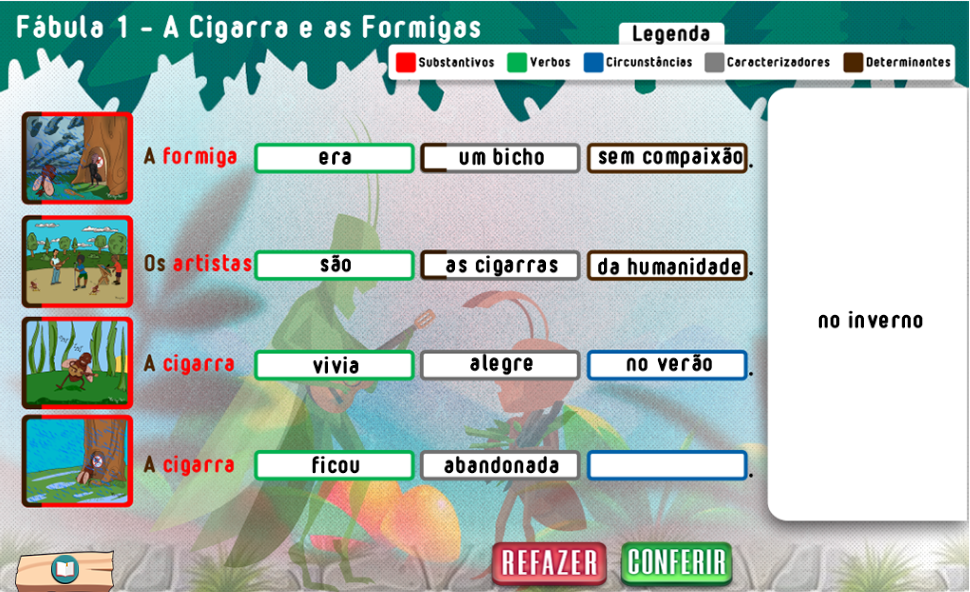
\includegraphics[width=\textwidth]{figure01.png}
\caption{Jogo Gramática das Fábulas: etapas e fábula.}
\label{fig:fig01}
\source{\hyperlink{http://www.wagnerodriguesilva.com.br/labgram}{http://www.wagnerodriguesilva.com.br/labgram}. }
\end{minipage}
\end{figure}

\begin{figure}[h] 
\centering
\begin{minipage}{.7\textwidth}
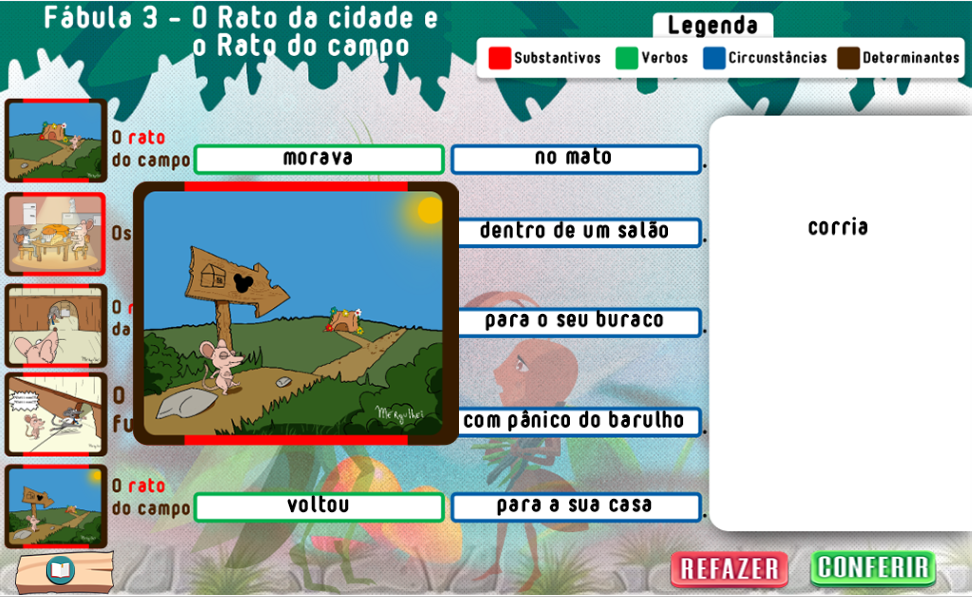
\includegraphics[width=\textwidth]{figure02.png}
\caption{Jogo Gramática das Fábulas: etapas e fábula.}
\label{fig:fig02}
\source{\hyperlink{http://www.wagnerodriguesilva.com.br/labgram}{http://www.wagnerodriguesilva.com.br/labgram}. }
\end{minipage}
\end{figure}

\begin{figure}[h] 
\centering
\begin{minipage}{.7\textwidth}
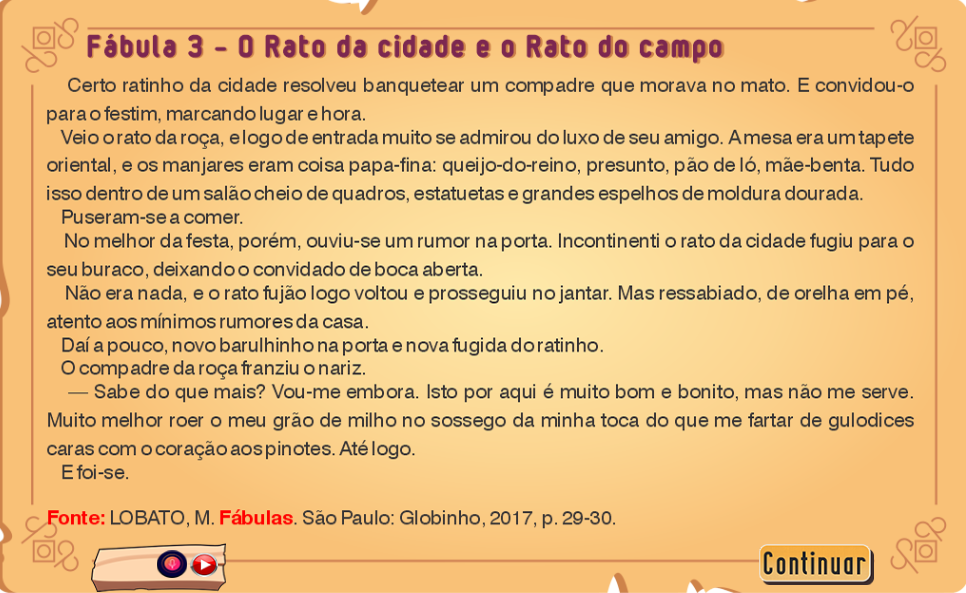
\includegraphics[width=\textwidth]{figure03.png}
\caption{Jogo Gramática das Fábulas: etapas e fábula.}
\label{fig:fig03}
\source{\hyperlink{http://www.wagnerodriguesilva.com.br/labgram}{http://www.wagnerodriguesilva.com.br/labgram}. }
\end{minipage}
\end{figure}

Em dissertação de mestrado, \textcite{ribeiro_producao_2021} identificou cinco aspectos
dinâmicos caracterizadores dos jogos e pensados coletivamente pelos
participantes do ConGraEduC, na produção colaborativa desses materiais
integrantes do LabGram. Com base nas Figuras \hyperref[fig:fig01]{1}, \hyperref[fig:fig02]{2} e \hyperref[fig:fig03]{3}, destacamos cada
aspecto ao analisarmos brevemente o jogo exemplificado:

\begin{enumerate}
\item Narrativa temática: auxilia na contextualização do objeto de
conhecimento gramatical trabalhado. O jogo trabalha a composição de
orações gramaticais, contextualizadas a partir de fábulas de Monteiro
Lobato. É composto por seis fases, cada uma com orações correspondentes
a um tipo verbal recontextualizado. As ilustrações 1 e 2 mostram a
primeira e terceira fases, que, respectivamente, focalizam as orações do
descrever e do agir. Para cada fase, é necessário ler e compreender uma
fábula para compor as orações.

\item Desafio: corresponde ao nível de dificuldade idealizado a depender
do objeto do conhecimento trabalhado e do público-alvo. O desafio maior
do jogo consiste na interpretação das fábulas, pois a montagem das
orações está condicionada principalmente à compreensão textual.

\item Autoexplicação: são jogos planejados para serem utilizados de forma
mais intuitiva. Os botões desenhados são icônicos: exibe fábula,
(des)aciona áudio, exibe ou oculta regras. Essas últimas são
apresentadas em textos curtos. O retorno ao texto de referência para
identificar informações necessárias à montagem das orações foi um
recurso bastante utilizado por estudantes.

\item Movimento: corresponde à disposição de elementos desencadeadores de
mobilidade, garantindo mais dinamismo. O jogo demanda que os usuários
arrastem os grupos gramaticais ou cliquem sobre as imagens com cenas da
narrativa para ampliá-las. Mensagens de erro ou de parabenização
aparecem ao final de cada fase ao ser acionado o botão de conferência. A
ampliação das imagens foi outro recurso bastante utilizado por
estudantes.

\item Multimodalidade: refere-se ao uso de diferentes linguagens para
contribuir com dinamismo do material. Está atrelado a quatro
subaspectos: escrita, oralidade, imagem e efeito sonoro. Áudios das
fábulas são disponibilizados e podem ser acionados a qualquer momento do
jogo. Ao final da fase, junto com a mensagem de acerto ou erro, aparece
um efeito sonoro característico do resultado alcançado. Uma música
instrumental pode ser acionada ou não durante o jogo, conforme
preferência do usuário. Além das imagens de fundo, que colaboram para
uma interação agradável, é utilizada uma imagem ampliável com alguma
cena da fábula como dica para a elaboração de cada oração.
\end{enumerate}


Com o uso dessa estratégia, os estudantes passaram a observar que o
funcionamento do conhecimento gramatical não se esgota no mero
reconhecimento de formas linguísticas, mas envolve, sobretudo, o
``desenvolvimento da capacidade de usar a linguagem para a troca de
significados'' \cite[p. 399]{hasan_literacy_1996}. Operando em conjunto, esses
aspectos dinâmicos do jogo didático potencializam a metalinguagem
funcional e, ao mesmo tempo, direcionam a atenção dos aprendizes para os
sistemas linguísticos em uso durante a leitura e a interpretação da
fábula.

Conforme observável nas legendas das Figuras \hyperref[fig:fig01]{1} e \hyperref[fig:fig02]{2}, foram padronizadas
cores para identificar os elementos gramaticais em posições específicas
na oração. Essa padronização fora empregada nos diferentes materiais do
LabGram. Utilizamos o vermelho para o substantivo núcleo do grupo
nominal na posição de participante principal; o verde para as diferentes
formas verbais; o rosa e o roxo para os substantivos complementos dos
verbos, sendo o último responsável pela função de beneficiário; o marrom
para os determinantes dos grupos nominais; o azul para as
circunstâncias; e o cinza para os substantivos ou adjetivos na posição
de participantes secundários em orações do descrever. O cinza também foi
utilizado para os elementos gramaticais na posição de atributos em
orações com processo material. Essas cores auxiliaram a escolha dos
grupos gramaticais a serem encaixados nos espaços sinalizados no jogo.

\phantomsection\label{anchor-6}{}

\begin{figure}[h]
\centering
\begin{minipage}{.7\textwidth}
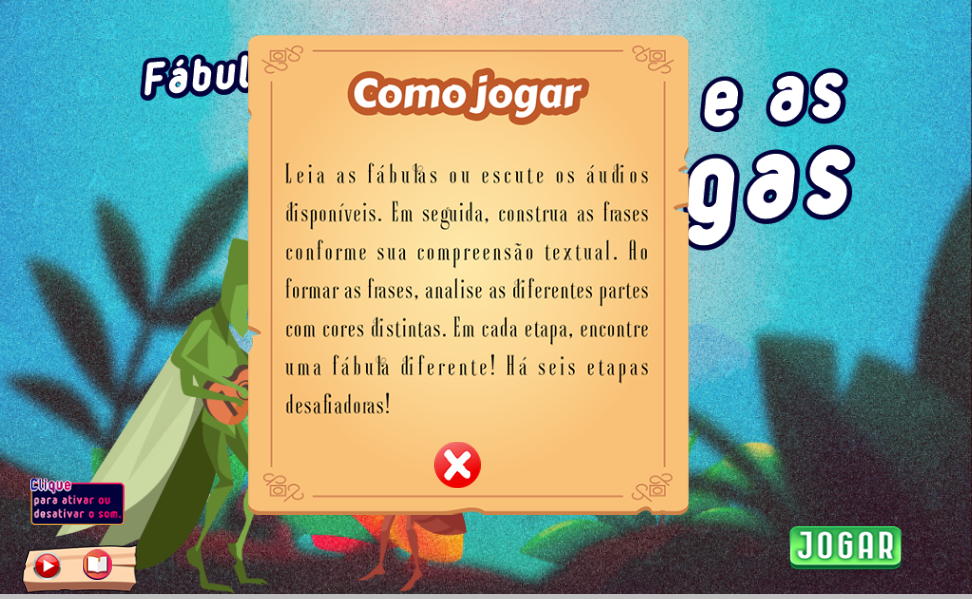
\includegraphics[width=\textwidth]{figure04.png}
\caption{Jogo Gramática das Fábulas: regra.}
\label{fig:fig04}
\source{\hyperlink{http://www.wagnerodriguesilva.com.br/labgram}{http://www.wagnerodriguesilva.com.br/labgram}. }
\end{minipage}
\end{figure}

\begin{figure}[h]
\centering
\begin{minipage}{.7\textwidth} 
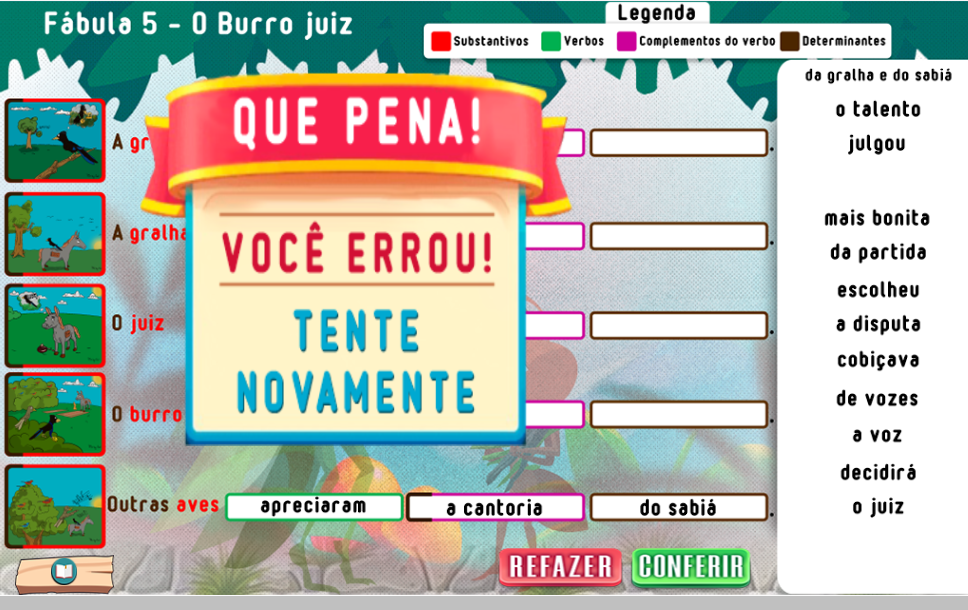
\includegraphics[width=\textwidth]{figure05.png}
\caption{Jogo Gramática das Fábulas: mensagem de erro.}
\label{fig:fig05}
\source{\hyperlink{http://www.wagnerodriguesilva.com.br/labgram}{http://www.wagnerodriguesilva.com.br/labgram}. }
\end{minipage}
\end{figure}

As expressões faceais espontâneas dos estudantes, captadas pela câmera
do Zoom e indicadas em parênteses duplos na interação transcrita,
revelam o engajamento deles ao refletirem sobre a língua durante a
execução do jogo. Foram utilizadas as seguintes convenções de
transcrição a partir de \textcite{preti_discurso_1999}: ( ) incompreensão de palavras ou
segmentos; (hipótese) hipótese do que se ouviu; MAIÚSCULA entonação
enfática; :: prolongamento da vogal ou consoante; - silabação; ...
qualquer pausa; ((minúscula)) comentários descritos do transcritor; -\/-
-\/- desvio da sequência temática; {[} sobreposição de falas; (...) fala
interrompida. A tais convenções, acrescentamos a seguinte: {[}...{]}
recorte do analista.

As professoras participantes, que também são coautoras deste artigo,
foram identificadas pelas iniciais dos seus dois primeiros nomes (KA e
AC). Os estudantes, por sua vez, foram identificados pelas seguintes
siglas fictícias: KS, linguista aplicado em atuação Kleber Silva; GR,
sociólogo Guerreiro Ramos (1915-1982); MS, geógrafo baiano Milton Santos
(1926-1921); e LB, socióloga gaúcha Luiza Bairros (1953-2016). Esses são
cientistas negros brasileiros aqui homenageados no esforço de
visibilizar outros grupos sociais, incluindo os profissionais atuantes
nas ciências humanas.

Visto que as orações gramaticais do jogo didático não estão explícitas
no texto, isso demandou uma leitura mais atenta da fábula e das imagens.
O \hyperref[tab-02]{Exemplo 1} do excerto de uma oficina de jogos mostra parte da
orientação inicial apresentada pela professora (AC), mais precisamente o
momento em que ela ressalta o auxílio das cores para o funcionamento do
jogo Gramática das Fábulas. Identificadas por legendas, há fases do jogo
com quatro e outras com cinco cores indicando distintas funções
gramaticais. Além de AC, participaram da interação dois estudantes
identificados pelas siglas fictícias KS e GR. Há referências também à
KA, professora da intervenção. Na referida oficina, esteve presente uma
servidora da instituição focalizada, ela observou a dinâmica da
atividade, mas não integrava a equipe do projeto.


\begin{table}[!htpb]
\centering
\small
	\begin{threeparttable}
		\caption*{\textbf{Exemplo 1.}}
		\label{tab-02}
		\begin{tabular}[]{@{} 
				>{\raggedright\arraybackslash}p{(\columnwidth - 0\tabcolsep) * \real{1.0000}}@{}}
			\toprule\noalign{}
			Oficina de jogo: legendas com cores 
			\\
			\midrule\noalign{}
			
			\textbf{127. AC:} {[}...{]} você tá vendo a legenda?
			
			\textbf{128. KS:} estamos
			
			\textbf{129. AC:} Dá uma olhadinha na legenda\ldots{}
			
			\textbf{130. KS:} Vermelho substantivo---
			
			\textbf{131. GR:} Verde... verbo... azul circunstância... cinza
			
			\textbf{132. AC:} caracterizadores
			
			\textbf{133. GR:} caracterizadores e marrom {[}
			
			\textbf{134. AC:} Determinantes ...vai \ldots{} chega um pouquinho o
			quadro de vocês ... Isso...Olha... aí você observa as cores... \emph{porque
				\emph{às vezes você pode fazer alguma mistura e olha o que tá te
					pedindo}}
			
			\textbf{135. KS: }humrum\textbf{ }((estudantes balançando a cabeça))
			
			\textbf{136. AC: }Então \emph{se eu colocar um substantivo aqui... eu já
					sei que não tá me pedindo um substantivo... nem a ordem é essa na
					frase}... Vamos lá... Olha pra imagem\ldots. Olha pra imagem olha pras
			palavras que você tem \ldots{} ((os estudantes estão pensando... põem a
			mão no queixo)) \phantomsection\label{anchor-7}{} \\
			\bottomrule
		\end{tabular}
	\end{threeparttable}
\end{table}


	Ao final do excerto reproduzido, a professora comentou sobre situações
	em que as cores legendadas podem auxiliar, pois os estudantes podem
	conseguir montar outras orações, diferentes das que foram planejadas.
	Esse movimento poderia ser evitado ao se observar as categorias
	gramaticais demandadas para os espaços identificados por cores (``às
	vezes você pode fazer alguma mistura e olha o que tá te pedindo''; ``se
	eu colocar um substantivo aqui... eu já sei que não tá me pedindo um
	substantivo... nem a ordem é essa na frase'').
	
	O \hyperref[tab-03]{Exemplo 2} mostra uma estratégia repetida pela professora, ao final de
	cada fase do Jogo Gramática das Fábulas. Antes de os estudantes
	arrastarem a última peça para completar a oração restante, quando
	automaticamente apareceria a mensagem de congratulação e mudaria para
	fase seguinte, AC fazia questionamentos sobre o tipo verbal trabalhado
	na fase concluída (``oh\ldots{} tremia... tonteou-se... assustou-se
	adormeceu e morreu é uma ação mental? (...) é uma ação involuntária?
	(...) é uma ação física?'').
	
\begin{table}[!htpb]
	\centering
	\small
	\begin{threeparttable}
		\caption*{\textbf{Exemplo 2.} }
		\label{tab-03}
		\begin{tabular}{@{} >{\raggedright\arraybackslash}p{(\columnwidth - 0\tabcolsep) * \real{1.0000}} @{}}
			\toprule\noalign{}
			Oficina de jogo: mediação da professora
			\\
			\midrule\noalign{}
			
			\textbf{287. AC:} Só uma perguntinha... olha-\/- pode colocar adormeceu-\/- Porque aí se tiver tudo certinho já vai fechar aí o jogo\ldots{} ((GR arrasta o verbo)) Deixa só eu perguntar pra vocês \\emph{oh\ldots{} tremia... tonteou-se... assustou-se adormeceu e morreu} ((KS inclinando olhar para AC)) \emph{É uma ação mental? (...) É uma ação involuntária? (...) É uma ação física?} ---
			
			\textbf{288. GR:} ((simulando tremor)) Tremia... acho que é uma ação involuntária\ldots{}
			
			\textbf{289. AC:} Olha aí pros verbos \ldots{}
			
			\textbf{290. KS:} tonteou-se... ((fazendo movimentos de dúvida com a boca e repetindo o verbo)) tonteou-se
			
			\textbf{291. GR:} ((inclina-se o corpo para o alto)) Tremia é uma ação involuntária que a gente num {[}
			
			\textbf{292. AC:} Olha aí pra esses verbos se eles são---
			
			\textbf{293. GR:} ((inclinando o olhar na direção de KS)) Tonteou- e \ldots{}
			
			\textbf{294. KS:} ((com a mão no queixo)) Pode ser também\ldots{}
			
			\textbf{295. AC:} Em que grupo eles estão?... É do agir do pensar ou do --- Tá certo ...Tonteou - se também
			
			\textbf{296. GR:} adormeceu e morreu também é uma ação involuntária
			
			\textbf{297. AC:} Então qual é o grupo aqui desses verbos?... Que grupo é esse?.... Do agir?... Do pensar?...
			
			\textbf{298. GR:} Do comportar\ldots{}
			
			\textbf{299. KS:} \emph{Do comportar\ldots{} nota 10 ... É isso aí} ((KS arrasta a palavra restante e encerra a fase 2 com a pontuação do JD))
			
			\textbf{300. AC:} Aeee\ldots((risos)) Gente vocês lembram que nós fizemos até uma atividade com esse não é?
			
			\textbf{300. GR:} Anram... com a KA\phantomsection\label{anchor-8}{} \\
			
			\bottomrule
		\end{tabular}
	\end{threeparttable}
\end{table}


	
	
	No contexto dessa interação, GR procurou relacionar as imagens do jogo
	com as informações lidas na fábula ``O peru medroso''. Diante das
	dificuldades iniciais dos estudantes em produzir as orações da fase 1,
	AC sugeriu que eles partissem da interpretação das imagens para chegar
	ao verbal. Ao observar GR descrevendo as etapas da narrativa a partir
	leitura dos desenhos, AC reforçou a contribuição da imagem para a
	execução do jogo (turno 228). Nessa fase foram explorados os verbos
	``tremia'', ``tonteou-se'', ``assustou-se'', ``adormeceu'', ``morreu'',
	formas de comportamento fisiológico e involuntário do peru e do galo
	diante das ameaças da raposa, personagens da narrativa temática do
	referido jogo.
	
	As reações dos estudantes indicam os esforços deles em pensar
	gramaticalmente \cite[]{halliday_grammar_2000}. Prova disso é que eles simularam as
	ações (``tremia...acho que é uma ação involuntária''), se inclinaram
	para argumentar (``tremia é uma ação involuntária que a gente num''),
	puseram a mão no queixo ao refletir sobre classificação (``pode ser
	também'') e riram das conclusões alcançadas (``adormeceu e morreu também
	é uma ação involuntária''). Esses gestos evidenciam o que diz Vigostski
	(2001, p. 110): ``a consciência reflexiva chega à criança através dos
	portais dos conceitos científicos''.
	
	De acordo com \textcite[p. 301]{halliday_hallidays_2014}, os verbos do
	comportar possuem limites indeterminados, apresentando características
	próximas das ações materiais, mentais e verbais, tal como evidenciam as
	reações dos estudantes no momento do jogo (``adormeceu'';
	``assustou-se''; ``morreu''; ``tonteou-se''; ``tremia''). Para imprimir
	às terminologias uma orientação semântica ainda mais precisa do que
	designamos aqui como \emph{verbos do comportar}, as imagens
	personalizadas ressaltaram expressões faciais e movimentos sinalizadores
	das ações involuntárias dos personagens, contribuindo com a
	interpretação textual. De alguma forma, a classificação de categorias
	gramaticais ainda se faz presente na prática da professora, conforme
	característico da tradição do ensino.
	
	Além dessas estratégias de recontextualização, as mediações realizadas
	por AC marcaram potencialmente o uso do jogo didático como espaço de
	troca e construção de saberes. Ao provocar situações pontuais de
	reflexão sobre a produção de sentidos dos tipos verbais
	recontextualizados nas orações, a professora ajudou o grupo de
	estudantes a caminhar na própria zona de desenvolvimento proximal (ZDP),
	conceito de \textcite{vigotski_construco_2001} que mobilizamos neste estudo para dar ênfase
	ao papel da mediação entre os conhecimentos espontâneos e científicos.
	Esse contexto interativo estabeleceu pontes entre o conteúdo gramatical
	e os aprendizes, favorecendo que os estudantes colocassem em ``jogo'' os
	conhecimentos prévios gerados no curso da própria atividade.
	
	Temos nessa situação de aprendizagem um movimento reflexivo e criativo
	que ultrapassa os limites do "codificado'', do foco em nomenclaturas e
	conceitos, permitindo ao estudante ``manipular o próprio material da
	linguagem, investindo-o de significação própria'' \cite[p.
	13]{franchi_criatividade_1987}. Não negamos que seja fundamental o estudante saber identificar e
	conceituar as categorias gramaticais, afinal, ``nomear os fenômenos é
	necessário para construção de qualquer saber científico'' \cite[p. 217]{mendonca_alise_2006}. Todavia, o ponto de partida consiste na associação das
	escolhas lexicais e gramaticais aos seus efeitos de sentido, trabalhando
	simultaneamente forma e significado, num trânsito constante entre
	atividades metalinguística e epilinguística. A recontextualização
	produtiva das terminologias numa perspectiva sistêmico-funcional fez do
	jogo um espaço para que os estudantes aprendessem a falar sobre a
	própria língua, descrevendo de forma sistematizada a funcionalidade de
	elementos linguísticos por meio de uma perspectiva reflexiva e
	consciente.
	
	Ao participarem dessa oficina de jogo, os estudantes permaneceram
	bastante envolvidos e entusiasmados, o que ficou perceptível nas
	distintas fisionomias, indicando concentração, reflexão e satisfação. Na
	seção focalizada, os estudantes queriam continuar jogando após o
	encerramento do horário da aula. O entusiasmo também foi inevitável por
	parte da professora, que vibrava até mais que os próprios estudantes a
	cada mudança de fase (``Do comportar\ldots{} nota 10 ... É isso aí
	{[}...{]} Aeee\ldots((risos))''). Ao final da intervenção, essa atitude
	foi recorrente por parte da referida professora, o que, talvez,
	justifique-se pela própria insegurança e desconfiança quanto à eficácia
	da inovação buscada, bastante evidente no início do projeto \cite{santos_construcao_2021}.
	
	Sobre esse contexto de interação, \textcite{gee_bons_2009} argumenta que boas
	experiências de aprendizagem são moldadas por meio atividades em que os
	sujeitos se engajam na realização de tarefas, interpretações,
	explicações, discussões e no próprio \emph{feedback} do jogo didático,
	do professor e dos colegas. Geradas por emoções positivas e por
	processos criativos propícios desse universo, essas situações
	interativas mediadas pelos jogos instauram um ambiente social e
	imaginário, que tendem a ser bastante satisfatórios para a construção da
	aprendizagem.
	
	Na seção seguinte, passamos a exemplificar evidências do aprendizado
	discente durante a intervenção pedagógica, o que é mostrado a partir da
	análise comparativa entre representações compartilhadas por dois
	estudantes antes e após a intervenção pedagógica.

\section{Transformação em aulas de língua materna}\label{sec-transformaçãoemaulasdelínguamaterna}

Analisamos o cruzamento de respostas compartilhadas por um mesmo
estudante para questionamentos semelhantes em duas entrevistas orais,
realizadas antes do início da intervenção e após sua conclusão.
Selecionamos pares de entrevistas de estudantes participativos nas
atividades desenvolvidas, e suas respostas são exemplares das falas de
outros colaboradores. Desta vez, utilizamos os nomes fictícios Milton e
Luiza para preservar as verdadeiras identidades de outros dois
estudantes e continuar homenageando cientistas negros brasileiros. A
análise recaiu sobre as seguintes temáticas: aulas de LP; gramática;
ciência; e pesquisa.

Conforme contrastes observáveis em diferentes excertos adiante, o
\hyperref[tab-04]{Exemplo 3} traz representações de aula de LP com perspectivas pedagógicas
distintas, sendo a intervenção responsável por resultados mais
produtivos. A monotonia das aulas fora representada na fala de Milton
com repetições lexicais descrevendo exercícios rotineiros copiados na
lousa em aulas de língua materna (``leitura e escrever leitura e
escrever''; ``só ler e escrever ler e escrever''). Esse tipo de aula foi
rotulado como ``meio chato''. Também reforçou essa monotonia o uso
exclusivo de livro didático em situações educativas do período pandêmico
(``basicamente usou só livro podemos se dizer'').


\begin{table}[!t] %Manter assim para melhor alinhamento - João 13/01/24
	\centering
	\small
	\begin{threeparttable}
		\caption*{\textbf{Exemplo 3.}}
		\label{tab-04}
		\begin{tabular}{@{} 
				>{\raggedright\arraybackslash}p{(\columnwidth - 2\tabcolsep) * \real{0.0300}} 
				>{\raggedright\arraybackslash}p{(\columnwidth - 2\tabcolsep) * \real{0.9700}} @{}}
			\toprule\noalign{}
			\multicolumn{2}{l}{Milton Santos: compreensão de aula de LP}  \\
			\midrule\noalign{}
			
			\multirow{6}{*}{\textbf{1ª}}   & \textbf{64. MS:} porque as minhas aulas de português são:: ficam \emph{meio chata} por quê? porque é só aquele negócio \emph{leitura e escrever leitura e escrever} entendeu? (...) \\
			
			&\textbf{65. KA: }sim \\
			
			&\textbf{66. MS: }aí isso vai dando uma preguiça da aula que (...) \\
			
			&\textbf{67. KA: }é verdade \\
			
			&\textbf{68. MS: }não tem nada diferente \emph{nunca tem nada diferente} é \emph{só ler e escrever ler e escrever} e\ldots{} \\
			
			&\textbf{217. MS:} sim basicamente \emph{usou só} livro podemos se dizer \\
            \midrule
			
			\multirow{3}{*}{\textbf{2ª }} & \textbf{148. MS:} SIM::: juro foi o que eu mais gostei de todo essa trajetória de vocês aqui...porque geralmente no ensino ... tradicional ... \emph{o ensino tradicional costuma dá... a questão e a resposta}... já na pesquisa de vocês estivemos que \emph{ir atrás da resposta}... não foi dada de mão beijada... e eu gostei pois \emph{desafiava a gente}... aquela coisa toda... \emph{a gente compreendia melhor} ... olha eu usando o a gente {[}...{]} \\
			
			&\textbf{165. KA:} você participaria de outra pesquisa como essa ... que a gente desenvolveu? \\
			
			&\textbf{166. MS:} SIM::... inclusive eu já iria falar ...\emph{se outra pesquisa dessa acontecesse atualmente ... nossa eu me empenharia  muito mais}... por que assim... vocês chegaram com a pesquisa ... no momento que eu tava... tão sabe... então em toda a pesquisa tava tendo um esforço a triplo pra fazer todas as coisas... agora atualmente ... eu digo que minha base de conhecimento ...aumentou um pouquinho pelo menos...e que é melhor em uma pesquisa \\
			
			\bottomrule
		\end{tabular}
	\end{threeparttable}
\centering
\end{table}



A monotonia comentada no primeiro excerto do \hyperref[tab-04]{Exemplo 3} parece retomada
na segunda entrevista, quando Milton caracteriza o ensino tradicional
pela reprodução de perguntas e respostas (``o ensino tradicional costuma
dá... a questão e a resposta''). Essa prática é contrastada com o
desafio e o aprendizado diferenciado trazidos pela pedagogia informada
por pesquisa do ConGraEduC (``já na pesquisa de vocês estivemos que ir
atrás da resposta... não foi dada de mão beijada... e eu gostei pois
desafiava a gente... aquela coisa toda... a gente compreendia melhor'').
Ao ser questionado sobre o interesse em participar de outra pesquisa
semelhante, o estudante demonstrou disposição para outras propostas
desafiadoras, afirmando se sentir mais preparado e em momento mais
propício para experiências do tipo, diferentemente do período pandêmico
(``se outra pesquisa dessa acontecesse atualmente ... nossa eu me
empenharia muito mais'').

No \hyperref[tab-05]{Exemplo 4}, o trabalho pedagógico com textos aparece como resposta
para questionamentos opostos, referentes às preferências e ao que menos
se aprecia em aulas de LP. Por um lado, a estudante valoriza a leitura
de textos em aulas (``os textos''). Provavelmente, esteja se referindo a
livros disponibilizados na biblioteca e lidos em algumas aulas, quando a
professora costumava solicitar resumos escritos sobre a narrativa. Por
outro lado, demonstra frustração com o que denomina de atividades com
textos, os quais não eram compreendidos por ela (``a gente não
compreende bem o texto e acaba ficando complicado responder as
atividades''). Certamente, esses efetivos exercícios escolares são
responsáveis por aulas monótonas, conforme já ilustrado na fala de
Milton.

\begin{table}[!htpb]
	\centering
	\small
	\begin{threeparttable}
		\caption*{\textbf{Exemplo 4.} }
		\label{tab-05}
		\begin{tabular}{@{} 
				>{\raggedright\arraybackslash}p{(\columnwidth - 2\tabcolsep) * \real{0.0300}} 
				>{\raggedright\arraybackslash}p{(\columnwidth - 2\tabcolsep) * \real{0.97000}} @{}}
			\toprule\noalign{}
			\multirow{2}{*}{Luiza Bairros: compreensão de aula de LP} \linebreak
			\\
			\midrule\noalign{}
			
			\multirow{8}{*}{1ª} & \textbf{35. KA: }ah perfeito... é:: e o que que você \emph{mais gosta nas aulas de língua portuguesa?} \\
			& \textbf{36. LB: }\emph{os textos} \\
			
			& \textbf{37. KA: }os textos? você gosta? é os textos que você lê que a professora leu os textos que você ouve que a professora é:: lê ... conta pra conta \\
			
			& \textbf{38. LB: }os dois \\
			
			& \textbf{39. KA:} é?.. beleza... O que você \emph{menos gosta nas aulas de língua portuguesa?} \\
			
			& \textbf{41. LB:} \emph{às vezes as atividades} \\
			
			& \textbf{42. KA:} e essas atividades incluem o quê? \\
			
			& \textbf{43. LB:} é que as vezes a gente \emph{não compreende bem o texto e acaba ficando complicado responder as atividades} \\
            \midrule
			
			\multirow{2}{*}{2ª} & \textbf{10. LB:} as aulas \emph{práticas ajudou bastante}... pra que a gente compreendesse melhor o conteúdo ... porque geralmente na sala de aula... é \emph{aquele conteúdo pratico né ...explica, explica}..... e o projeto de vocês .... foi muito é:: \emph{JOGOS É: AULA PRÁTICAS mesmo} .... e isso ajudou bastante o conhecimento {[}...{]} \\
			
			& \textbf{40. LB:} ((risos)) porque com os jogos a gente geralmente a gente está ... \emph{naquela expectativa} ... ah eu preciso ganhar eu quero ganhar e tal e.... acaba que \emph{a gente tem uma empolgação maior e acaba se empenhando mais} ... pra fazer aquele jogo ... eu quero ganhar e tal ... \emph{aí acaba que a gente se concentrando mais... e isso ajuda a gente aprender mais a raciocinar} \\
			
			\bottomrule
		\end{tabular}
	\end{threeparttable}
\end{table}


As aulas ministradas na intervenção foram caracterizadas como práticas e
contrapostas ao que Luiza denominou de ``conteúdo prático'', certamente
uma escolha lexical inadequada, no momento inicial da entrevista, quando
a estudante demonstrava nervosismo. Ao assistirmos ao registro em vídeo,
compreendemos que, certamente, Luiza aludia a ``conteúdo teórico''.
Assim, estaria se referindo a aulas expositivas monótonas, sinalizadas
pela repetição lexical (``explica, explica''). A escolha lexical
``mesmo'' e a ênfase entonacional também contribuíram para se contrapor
a uma suposta monotonia (``JOGOS É: AULA PRÁTICAS mesmo'').


Enquanto Milton realçou o papel de práticas de pesquisa em sala de aula,
Luiza destacou a relevância dos jogos didáticos digitais (``e isso
ajudou bastante o conhecimento''). Conforme Luiza, os jogos provocam uma
série de emoções nos estudantes, colaborando para o engajamento nas
atividades pedagógicas (``naquela expectativa ... ah eu preciso ganhar
eu quero ganhar e tal e.... acaba que a gente tem uma empolgação maior e
acaba se empenhando mais ... pra fazer aquele jogo ... eu quero ganhar e
tal ... aí acaba que a gente se concentrando mais... e isso ajuda a
gente aprender mais a raciocinar'').

A respeito das representações sobre gramática, o desconhecimento do
assunto foi verbalizado pelos colaboradores. No primeiro excerto da
entrevista do \hyperref[tab-06]{Exemplo 5}, a negativa se mostra recorrente na interação. O
desconhecimento se torna marcado quando Milton afirma que o estudo da
gramática ocorreu no passado, ignorando sua constante presença em aulas
de LP (``creio que estudei há muitos anos atrás''). Em resposta à
insistência da professora para que o estudante saísse da negação, Milton
equivocadamente faz referência a textos em quadrinhos, que tinham
presença garantida em aulas de LP frequentadas por ele (``mas é algo
relacionado a histórias do tipo HQ em um livro sei lá'').

\begin{table}[htpb]
\caption{Quadro comparativo.}
\label{tab06}
\centering
\begin{tabular}{@{}lll@{}}
\toprule 
  & Segundo AGV & Primeiro AGV \\
\midrule
Raio da roda traseira & 2,5cm & 2,37cm \\
Comprimento de arco da roda & 15,7cm & 14,9cm \\
Rotação da roda (matematicamente) & 245RPM & 230RPM \\
Velocidade roda & 3.846cm/min & 3.427cm/min \\
Velocidade média no percurso & 3.000cm/min & 2.861cm/min \\
Média de rotações da roda (empiricamente) & 191RPM & 192RPM \\
Peso & 230g & 217g \\
\bottomrule
\end{tabular}
\source{Acervo dos autores.}
\end{table}




\phantomsection\label{anchor-10}{}

No \hyperref[tab-06]{Exemplo 5}, o excerto da segunda entrevista revela um estudante seguro
para compartilhar conhecimentos apropriados sobre gramática, inclusive
preocupado em evitar minimizar a relevância do trabalho interventivo
realizado (``se minha resposta não for o que você está esperando... não
é culpa de vocês e nem NADA ... por que eu aprendi muita coisa durante
isso''). Milton compartilhou uma compreensão funcional de gramática.
Seria composta por regras responsáveis pela composição textual (``é um
conjunto de regra que pode ditar como a estrutura de um texto funciona
... para que ele seja compreensível ... essa é a base de uma coisa bem
mais resumida o que é gramática''). Ao ser provocado pela professora, o
estudante reitera o distanciamento de uma suposta concepção de gramática
normativa, ao explicitar a noção de adequação dos usos da língua,
realçando a relevância do registro formal, especialmente no domínio
acadêmico (``funcionamento ... até porque não existe certo ou errado...
existe adequado e inadequação'').

O primeiro excerto do \hyperref[tab-07]{Exemplo 6} ilustra o desconhecimento discente a
respeito da gramática. Assim como visto no exemplo anterior, as
negativas são recorrentes nas respostas de Luiza (``eu não sei bem o que
que é''; ``não não que eu lembre''; ``pra falar a verdade eu não sei
muito bem o que é isso''). Esse momento inicial pode se caracterizar
como um esquecimento, ao considerarmos o segundo excerto reproduzido,
uma vez que, ao final da intervenção pedagógica, Luiza consegue
compartilhar alguma lembrança de um trabalho gramatical prescritivo e
constante (``a gente estudava muito ... a gramática era dada pra::...
pra dar ordem acho que era para dar ordem se não me engano ao texto'').

\begin{table}[!t] %Manter assim para melhor alinhamento - João 14/01/24
	\centering
	\small
	\begin{threeparttable}
		\caption*{\textbf{Exemplo 6.}}
		\label{tab-07}
		\begin{tabular}{@{} 
				>{\raggedright\arraybackslash}p{(\columnwidth - 2\tabcolsep) * \real{0.0300}} 
				>{\raggedright\arraybackslash}p{(\columnwidth - 2\tabcolsep) * \real{0.97000}} @{}}
			\toprule\noalign{}
			\multirow{2}{*}{Luiza Bairros: compreensão de gramática} \linebreak
			\\
			\midrule\noalign{}
			
			\noalign{}
			
			
			\textbf{1ª} & \textbf{61. LB: }hum... algumas vezes mas eu \emph{não sei bem o que que é} \\
			
			& \textbf{76. KA: }sim com as suas palavras o que você entende por gramática? você já estudou gramática você estudou isso na escola? \\
			
			& \textbf{77. LB: }\emph{não} \\
			
			& \textbf{78. KA: }\emph{nunca} estudou isso na escola? \\
			
			& \textbf{79. LB:} \emph{não não} que eu lembre {[}...{]} \\
			
			& \textbf{85. KA:} pra falar a verdade eu \emph{não sei muito bem} o que é isso \\
            \midrule
			
			\textbf{2ª } & \textbf{54. LB:} a gente estudava muito ... a gramática era dada pra::... pra dar ordem acho que era para dar ordem se não me engano ao texto ... enfim não estou lembrando muito .... mas agora depois do projeto deu pra entender que:.... \emph{a gramática ela tá pra dá sentido ao texto à fala ou algo...que está sendo mostrada} \\
			\bottomrule
		\end{tabular}
	\end{threeparttable}
\end{table}




Após a vivência da intervenção pedagógica, Luiza relaciona a gramática à
construção de sentido de textos escritos ou falados, portanto também se
distancia da concepção prescritiva comumente trabalhada em escolas
(``mas agora depois do projeto deu pra entender que:.... a gramática ela
tá pra dá sentido ao texto à fala ou algo...que está sendo mostrada'').

Ao ser questionado sobre o que compreendia por ciências, na entrevista
inicial, MS reconheceu a relevância da ciência (``eu sempre coloco
ciência acima de tudo''; ``primeiro algo necessário''), ainda que tenha
demonstrado dificuldade para elaborar um conceito propriamente dito. O
\hyperref[tab-08]{Exemplo 7} mostra que o estudante fez referência ao contexto da pandemia,
para ilustrar a importância da ciência em momentos difíceis, podendo
minimizar o sofrimento humano em geral (``bora fingir que não existe a
ciência um exemplo pro que nós tamo passando agora... qual qual outros
meio nós iria usar? sobrenatural? crença?''). Talvez sob a influência de
discursos negacionistas propagados durante a pandemia, Milton explicitou
a irritação com a tendência de se misturarem crenças e ciência, ainda
que compartilhe as próprias crenças (``eu tenho muita crença em certas
coisas mas aí gente me subornam\footnote{ Possivelmente, a escolha
	lexical empregada foi inapropriada, já que o estudante faz referência
	às pessoas que tentam convencê-lo a acreditar nas crenças religiosas
	em detrimento dos fatos científicos. Certamente, a palavra poderia ser
	substituída por ``subestimam''.} demais falam que qualquer coisa é só
crença é só crença... ah eu acredito em tal crença tal Deus meu vai
fazer tal coisa assim... e de me misturar até a crença junto com a
ciência entendeu?''; ``não isso me irrita''). A representação de ciência
compartilhada no exemplo parece circunscrita aos conhecimentos
legitimados pela tradição científica, sem margens para saberes
alternativos.


\begin{table}[h]
	\centering
	\small
	\begin{threeparttable}
		\caption*{\textbf{Exemplo 7.} }
		\label{tab-08}
		\begin{tabular}{@{} 
				>{\raggedright\arraybackslash}p{(\columnwidth - 2\tabcolsep) * \real{0.0300}} 
				>{\raggedright\arraybackslash}p{(\columnwidth - 2\tabcolsep) * \real{0.9700}} @{}}
			\toprule\noalign{}
			\multirow{2}{*}{Milton Santos: compreensão de ciência}
			
			\\
			\midrule\noalign{}
			
			
			
			
			\textbf{1ª } & \textbf{218. KA.} {[}...{]} a outra pergunta essa também é pessoal tá Milton? É o que você acha ne? É o que você compreende... é é... o que você compreende por ciência? quando vem a palavra ciência na sua cabeça o quê que você entende?... não é a resposta certa que eu estou querendo eu estou querendo ver o que você entende \\
			
			& \textbf{219. MS:} ~até porque eu \emph{não ia saber dar} ela né? ((rindo)) {[}...{]} \\
			
			& \textbf{223. MS:} ~humm olha assim... eu tenho eu sempre nossa... eu vou uma coisa pessoal aqui exemplo eu tenho muita coisa tipo \emph{eu sempre coloco ciência acima de tudo não em certas coisas do tipo bora se dizer que:: ciência pra mim é::... é:: como eu posso explicar gente... ((pensando)) gente sem palavras sem reação}... pera {[}...{]} \\
			
			& \textbf{228. KA: }nas suas palavras é o que? nas suas palavras é o que? quando vem a palavra ciência na sua cabeça o quê que o quê que vem à mente? \\
			
			& \textbf{229. MS:} ~\emph{primeiro algo necessário} \\
			
			& \textbf{230. KA: }aham \\
			
			& \textbf{231. MS:} ~porque assim gente bora fingir que não existe a ciência um exemplo pro que nós tamo passando agora... qual qual outros meio nós iria usar? \emph{sobrenatural?} \emph{crença?} \\
			
			& \textbf{232. KA: }ah ((ri)) muito bem:: exatamente então \\
			
			& \textbf{233. MS:} ~-\/- eu tenho... eu tenho uma que eu consigo eu sou eu tenho muita crença em certas coisas mas ai gente me subornam demais falam que qualquer coisa é só crença é só crença... ah eu acredito em tal crença tal Deus meu vai fazer tal coisa assim... e de me \emph{misturar até a crença junto com a ciência entendeu}? e e:: \\
			
			& \textbf{234. PD: }e você concorda com isso? \\
			
			& \textbf{235. MS:} ~\emph{não isso me irrita} \\
			
			& \textbf{236. PD: }por quê? \\
			
			& \textbf{237. MS:} ~porque assim eu acho exemplo... a chuva \\
			
			& \textbf{238. PD: }aham \\
			
			& \textbf{239. MS:} ~tem gente que chegou em mim e falou que tal pessoa lá em cima fez chover... \emph{não no meu caso já é o que ciência mostra entendeu}? \\
            \midrule
			
			\textbf{2ª} & \textbf{132. MS:} oh... uma coisa que eu descobri que foi \emph{um BUM} ... foi que \emph{vocês quebraram uma barreira que tinha em mim} ... sobre esse negócio de ciência... quando falou que iriamos \emph{fazer uma pesquisa cientifica da linguagem... fiquei tipo... QUE? COMO ASSIM?}... pois na minha cabeça infantil ainda...tinha aquele negócio de \emph{carinha de cabelo bagunçado}... \emph{aquele branquelo}... estadunidense e tudo mais... com aqueles vidros e tal ... mas... sobre ciência eu digo que é \emph{uma área que abrange ... basicamente tudo... que pode ser estudada e experimental .... tem o exemplo das linguagens também} \\
			\bottomrule
		\end{tabular}
	\end{threeparttable}
\end{table}


\phantomsection\label{anchor-12}{}


A intervenção pedagógica contribuiu para ampliar a visão de ciência
compartilhada por Milton (``sobre ciência eu digo que é uma área que
abrange ... basicamente tudo... que pode ser estudada e experimental
.... tem o exemplo das linguagens também''), conforme segundo excerto do
\hyperref[tab-08]{Exemplo 7}. O estudante desconhecia a prática científica nas ciências da
linguagem, pois tal descoberta foi descrita como uma quebra de barreira
(``que foi um BUM ... foi que vocês quebraram uma barreira que tinha em
mim''; ``quando falou que iriamos fazer uma pesquisa cientifica da
linguagem... fiquei tipo... QUÊ? COMO ASSIM?''). A representação prévia
compartilhada correspondia à imagem de um cientista branco de cabelo
bagunçado, provavelmente uma imagem masculina e estrangeira (``na minha
cabeça infantil ainda...tinha aquele negócio de carinha de cabelo
bagunçado... aquele branquelo... estadunidense'').


O \hyperref[tab-09]{Exemplo 8} apresenta uma concepção restrita de ciência, compartilhada
por Luiza antes da intervenção pedagógica. Limitava-se a disciplinas
escolares, especialmente a Ciências Naturais, estudam-se ``animais'' e o
``corpo humano'' (``muita matéria'', ``é tudo né mais ou menos... é::
animais faz parte das ciências essas coisas''; ``exatamente específico
para uma disciplina ...''). A estudante demonstra ter ampliado a
representação de ciência a partir da intervenção; o processo de
construção e de apropriação do conhecimento foram significativos na
experiência vivenciada (``e agora com todo o projeto todo estudo ... a
gente entendeu que a ciência num é ... só voltada a uma disciplina'';
``porque a gente estuda e no final a gente adquiri um conhecimento'').
Certamente, contribuiu também o fato de Luiza ter atuado como bolsista
de iniciação científica júnior no ConGraEduC.

\begin{table}[!t] %Manter assim para melhor alinhamento - João 14/01/24
	\centering
	\small
	\begin{threeparttable}
		\caption*{\textbf{Exemplo 8.} }
		\label{tab-09}
		\begin{tabular}{@{} 
				>{\raggedright\arraybackslash}p{(\columnwidth - 2\tabcolsep) * \real{0.0300}} 
				>{\raggedright\arraybackslash}p{(\columnwidth - 2\tabcolsep) * \real{0.9700}} @{}}
			\toprule\noalign{}
			\multirow{2}{*}{Luiza Bairros: compreensão de ciência}
			\linebreak
			\\
			\midrule\noalign{}
			
			\noalign{}
			
			
			\textbf{1ª } & \textbf{128. KA:} quando vem na sua cabeça -\/- espontâneo assim quando é espontâneo quando você quando você vem alguém fala a palavra ciência isso é uma coisa é:: da ciência o que que vem na sua cabeça? \\
			
			& \textbf{129. LB:} vem \emph{muita matéria} né? \\
			
			& \textbf{130. KA: }{[}a matéria {[} \\
			
			& \textbf{131. LB:} a matéria de ciência \\
			
			& \textbf{132. KA:} \emph{é?} \\
			
			& \textbf{133. LB:} ((olhando para o alto com mão na cabeça e pensando)) é ciência é tudo... né? -\/- mais ou menos... é:: animais faz parte da ciências essas coisas... né? \\
            \midrule
			
			\textbf{2ª } & \textbf{98. LB:} \emph{é o conhecimento}! ((sorrindo))... que \emph{a gente estuda para ter um certo conhecimento} ... \emph{no final adquirimos conhecimento} ... antes nas aulas normais ... \emph{a ciência estava voltada ao corpo humano a essas coisas do tipo}...e... \\
			
			& \textbf{99. AC:} mais especifico uma disciplina \\
			
			& \textbf{100. LB:} isso:... \emph{exatamente específico para uma disciplina} ... e agora com todo o projeto todo estudo ... \emph{a gente entendeu que a ciência num é ... só voltada a uma disciplina ... mas sim voltada ao conhecimento ... porque a gente estuda e no final a gente adquiri um conhecimento} \\
			\bottomrule
		\end{tabular}
	\end{threeparttable}
\end{table}

\phantomsection\label{anchor-13}{}

É interessante observar que, inicialmente, os estudantes focalizados não
associam as noções de ciência e de pesquisa, quando são questionados
sobre tais atividades. Conforme \hyperref[tab-10]{Exemplo 9}, Milton se refere à pesquisa
como uma prática escolar corriqueira de procura por informação sobre
algo ignorado, a exemplo da busca na internet por significado de
palavras desconhecidas (``sempre que eu num sei de nada eu vou pesquisar
uma palavra eu num conheço ela eu vou pesquisar sobre essa palavra''). A
pesquisa escolar também é referenciada quando o estudante se recorda de
uma pesquisa sobre insetos, realizada para uma exposição presencial numa
aula de Ciências Naturais, quando precisou se caracterizar do próprio
inseto pesquisado. A lembrança fez Milton recordar de equipamentos
especiais disponibilizados na escola para atividades nessa área do
conhecimento, a exemplo de binóculos e microscópios.


\begin{table}[!t] %Manter assim para melhor alinhamento - João 14/01/24
	\centering
	\small
	\begin{threeparttable}
		\caption*{\textbf{Exemplo 9.} }
		\label{tab-10}
		\begin{tabular}{@{} 
				>{\raggedright\arraybackslash}p{(\columnwidth - 2\tabcolsep) * \real{0.0300}} 
				>{\raggedright\arraybackslash}p{(\columnwidth - 2\tabcolsep) * \real{0.9700}} @{}}
			\toprule\noalign{}
			\multirow{2}{*}{Milton Santos: compreensão de pesquisa}
			\linebreak
			 \\
			\midrule\noalign{}
			
			
			
			
			\textbf{1ª } & \textbf{253. MS:} {[}...{]} \emph{sempre que eu num sei de nada eu vou pesquisar uma palavra eu num conheço ela eu vou pesquisar sobre essa palavra} aí conheço sobre essa palavra e aí pronto eu já sei tá eu sei o que é isso... então em certa ocasião falam isso eu não vou precisar mais pesquisar mais através da pesquisa eu conheci o que era ela entendeu? \\
			
			& \textbf{254. KA:} exatamente... é:: a última pergunta... você já participou de alguma atividade de pesquisa na escola? {[}...{]} \\
			
			& \textbf{255. MS:} ~nossa...há 4 anos atrás sim {[}...{]} \\
			
			& \textbf{274. MS:} ~e... é só foi tipo a gente ficou com a missão de fazer uma pesquisa... o nosso foi sobre insetos e eu pesquisei sobre a joaninha... eu nem sei basicamente eu nem vejo mais joaninha hoje em dia qualquer eu nem saio do quarto então eu nem vejo joaninha {[}...{]} \\
			
			& \textbf{284. MS: }e também na na minha esco agora que eu tô lembrando que \emph{na minha escola tinha alguns objetos que a gente devia usar... num tem?... tipo binóculos essas coisas do tipo} \\
            \midrule
			
			\textbf{2ª } & \textbf{138. MS:} oh assim... pesquisa é \emph{um processo de investigação em determinado tema... onde você vai na raiz do problema...até chegar quase em uma conclusão de resolver ou resolver...que passa por uma longa etapa de coisa} \\
			
			& \textbf{139. KA:} exato... você experenciou isso... né? \\
			
			& \textbf{140. MS:} sim\phantomsection\label{anchor-14}{}\phantomsection\label{anchor-15}{}\phantomsection\label{anchor-16}{} \\
			
		\end{tabular}
	\end{threeparttable}
\end{table}


Com a intervenção pedagógica, a compreensão de pesquisa foi ampliada.
Milton passou a fazer referência à possibilidade de resolução de
problemas a partir de um processo investigativo criterioso (``você vai
na raiz do problema...até chegar quase em uma conclusão de resolver ou
resolver...que passa por uma longa etapa de coisa''), que corresponde
exatamente à vivência experienciada por ele com as atividades educativas
do ConGraEduC. Essa mesma ideia de percurso, trajetória e processo fora
explicitada por Luiza na segunda entrevista, ao ser igualmente
questionada sobre pesquisa, conforme segundo excerto do \hyperref[tab-11]{Exemplo 10}.

\begin{table}[!htpb]
	\centering
	\small
	\begin{threeparttable}
		\caption*{\textbf{Exemplo 10.} }
		\label{tab-11}
		\begin{tabular}{@{} 
			>{\raggedright\arraybackslash}p{(\columnwidth - 2\tabcolsep) * \real{0.0300}} 
			>{\raggedright\arraybackslash}p{(\columnwidth - 2\tabcolsep) * \real{0.9700}} @{}}
			\toprule\noalign{}
			\multirow{2}{*}{Luiza Bairros: compreensão de pesquisa} \linebreak \\
			\midrule\noalign{}
			
			
			
			
			\textbf{1ª} & \textbf{171. LB:} \emph{buscar informação... saber mais sobre o assunto} {[}...{]} \\
			
			& \textbf{185. LB: }sim às vezes ela coloca por exemplo ela coloca assim é::... faça alguma coisa \emph{faça uma pesquisa sobre a guerra mundial a gente vai lá e pesquisa é::... guerra mundial e vai aparecer um textão né a gente vai ler resumir e fazer} \\
			
			& \textbf{186. KA: }ah muito bem {[}...{]} \\
			
			& \textbf{187. LB: }é isso  \\
            \midrule
			
			\textbf{2ª } & \textbf{102. LB:} a pesquisa é todo o \emph{percurso} ... que a gente \emph{percorre} é::: estudando livros ...tal ... então resumindo ... pesquisa é todo o \emph{percurso} ... toda uma \emph{trajetória} que a gente faz para chegar a um certo resultado ... \phantomsection\label{anchor-17}{} \\
			\bottomrule
		\end{tabular}
	\end{threeparttable}
\end{table}


Uma compreensão escolarizada de pesquisa também é compartilhada no
\hyperref[tab-11]{Exemplo 10}, quando Luiza descreve o tipo de exercício proposto em sala
de aula (``buscar informação''). Trata-se do comando para a busca
informações sobre uma temática aberta, normalmente escolhida por
professores, para que sejam produzidos resumos a partir de extensos
textos disponíveis na internet (``faça uma pesquisa sobre a guerra
mundial a gente vai lá e pesquisa é::... guerra mundial e vai aparecer
um textão né a gente vai ler resumir e fazer''). Infelizmente, esses
resumos tendem a se configurar na justaposição de excertos copiados, não
resultantes do efetivo trabalho cognitivo de compreensão e elaboração
textual passível de reescrita.

\section{Considerações finais}\label{sec-consideraçõesfinais}

A interação entre as comunidades escolar e universitária se mostrou
produtiva pelo fato de as pessoas envolvidas poderem experienciar
processos colaborativos de produção do conhecimento. Isso se desdobrou
em ganhos imediatos, a exemplo:
\begin{enumerate}[label=\alph*)]
\item da visibilização, por parte das
professoras, da prática científica pulsante no próprio local de
trabalho, onde diariamente se precisa construir a inovação do ensino de
língua materna; \item e da transformação de representações equivocadas,
compartilhadas por estudantes colaboradores, resultado de uma tradição
ineficiente do ensino.
\end{enumerate}
 Diferentemente da imagem de pesquisa relacionada
à simples cópia de informações aleatórias a partir de livros ou páginas
da internet, e de ciência meramente associada à disciplina escolar ou
silenciada por crenças, a intervenção pedagógica mediada por práticas
investigativas pertinentes ressignificou parte dessas representações ou
entendimentos equivocados.

Assim como proporcionado por outros materiais didáticos produzidos no
ConGraEduC, o jogo Gramática das Fábulas colocou os estudantes em
situações educativas de experimentação da reflexão \emph{com} e
\emph{sobre} a gramática da língua materna, prática até então
desconhecida dos referidos colaboradores, conforme comumente observável
em escolas brasileiras. A experimentação dessa prática se faz necessária
numa abordagem da educação científica, que trabalha com situações de
investigação sobre a língua, as quais são efetivas atividades de análise
linguística, quando também se empregam terminologias, conforme
característico do trabalho científico.

Conforme demonstrado nas análises dos dados, o conhecimento mediado pelo
jogo didático digital auxiliou os estudantes a lidarem com a língua como
objeto de investigação, compreendendo-a em seus modos de significar,
naturalmente articulados a experiências interativas do cotidiano. Assim,
posicionados ativamente pelo próprio contexto do jogo e as mediações
realizadas pelas professoras, esses estudantes se engajaram em
experiências de aprender fazendo, refletindo, levantando hipóteses,
buscando soluções, formulando e reformulando construções linguísticas,
exercitando etapas que integram as competências básicas de atividades
investigativas. São justamente iniciativas desse tipo que favoreceram a
promoção da alfabetização e do letramento científicos, também, em aulas
de LP\footnote{Agradecemos a Profa. Dra. Mirella de Oliveira Freitas
	(UFU) pela leitura crítica realizada de uma versão preliminar deste
	artigo, os possíveis equívocos restantes são de inteira
	responsabilidade das autoras e do autor.}.
	
	
\section{Agência financiadora}\label{sec-agênciafinanciadora}
Agradecemos ao governo federal brasileiro, aqui representado pelo
Conselho Nacional de Desenvolvimento Científico e Tecnológico (CNPq),
pelo financiamento do projeto Conscientização Gramatical pela Educação
Científica -- ConGraEduC (Proc. ~441194/2019-2). O primeiro autor deste
artigo agradece ainda à mesma agência de fomento pela bolsa de
produtividade em pesquisa -- PQ/1D (Proc. 304186/2019-8).
